
\chapter{Introducción}


En la actualidad la extracción de conocimiento sobre datos está
adquiriendo cada vez más una mayor relevancia en el campo de la
ciencia de la computación y, con ello, una mayor aplicación en el
mundo industrial y empresarial. Este crecimiento se traduce en la
necesidad de investigación e innovación en las técnicas de minería
de datos.


En concreto, la detección de anomalías surge como un problema
específico, pero a la vez de gran relevancia, que consiste en la
identificación de aquellas instancias del conjunto de datos que,
debido a que se desvían del resto, se convierten en un caso con
un gran interés.

Un importante enfoque para la detección de anomalías es el basado
en la idea de proximidad, por el que consideraremos que una instancia
es una anomalía si es similar a las instancias que se encuentran
próximas \cite{aggarwalOutlierAnalysis2017}.  Se considerarán tanto técnicas basadas en
clustering, donde se identifica como instancias anómalas aquellas
que se sitúan en pequeños clústeres o se encuentran alejadas del
clúster al que se han asignado; las basadas en distancias y en técnicas
como el k-NN \cite{ishimtsevConformalKNNAnomaly2017}; y las técnicas basadas en densidad,
donde interviene el número de puntos existentes en una región local.

En este proyecto proponemos la realización de una biblioteca en Python
de métodos de detección de anomalías basados en proximidad, así como
la comparación de su eficacia en distintos ámbitos y la eficiencia de
estos métodos.



\section{¿Qué es una anomalía?}
Una anomalía es un punto de datos que es significativamente diferente
de los datos restantes. Hawkins definió [249] un valor atípico de la siguiente manera:



\textit{
 ``Una anomalía es una observación que se desvía tanto de las
otras observaciones como para despertar sospechas de que fue generado
por un mecanismo diferente"}


Como podemos ver este problema es realmente interesante y tiene un alto valor,
como nos menciona \textbf{Eugene Nathaniel Butler} \cite{quotationsEugeneNathanielButler}, estos casos especiales,
o diferentes pueden ser los más importantes.

\textit{
``Nunca tome el comentario de que usted es diferente como una condena,
podría ser un cumplido. Podría significar que posees cualidades únicas
que, como el más raro de los diamantes, es... único en su clase."}

En la minería de datos podemos encontrar diferentes términos para referirnos
a una anomalía como valor atípico, discordante,
desviaciones o datos fuera de lo normal. Cuando tomamos datos de una aplicación
podemos recibir información de uno o más procesos de generación,
lo cual puede reflejarse en la actividad del sistema y en las observaciones recopiladas.
Cuando el proceso de generación se comporta de manera inusual, resulta en la creación de anomalías.
Por lo tanto, un valor atípico a menudo contiene información muy útil sobre propiedades
anormales de los sistemas y entidades que afectan el proceso de generación de datos.
La detección de tales características inusuales proporciona información útil y específica de la aplicación.
La aplicación de la detección de anomalías puede aplicarse a numerosos campos como los siguientes:

\begin{itemize}
    \item \textbf{Sistemas de detección de intrusos.} En los sistemas informáticos, se recopilan diferentes
    tipos de datos como las llamadas del sistema operativo, el tráfico de la red u otras acciones de los usuarios.
    Estos datos pueden mostrar un comportamiento extraño debido a la actividad maliciosa. El reconocimiento de dicha
    actividad puede ser clave para evitar problemas mayores \cite{kumarAnomalyBasedNetworkIntrusion2019}
    \cite{jabezIntrusionDetectionSystem2015}.
    \item \textbf{Diagnóstico médico.} En la mayoría de aplicaciones médicas, los datos se recopilan de una variedad
    de dispositivos, como las imágenes por resonancia magnética (IRM), la tomografía por emisión de positrones (PET)
    o las series cronológicas de electrocardiogramas (ECG). Detectar patrones inusuales en tales datos, nos ayudará a
    detectar enfermedades
    \cite{vIdentificationOutliersMedical2014} \cite{gasparSystematicReviewOutliers2011}.
    \item \textbf{Fraude con tarjetas de crédito.} El fraude con tarjetas de crédito se ha vuelto un problema latente
    en nuestra sociedad, debido a la mayor facilidad con que la información confidencial, como el PIN de una tarjeta de crédito,
    puede verse comprometido. En la mayoría de casos, el uso no autorizado de una tarjeta de crédito puede mostrar diferentes patrones,
    como la compra desde ubicaciones particulares o transacciones muy grandes. Dichos patrones pueden usarse para detectar
    anomalías en los datos de transacciones y evitar dichos fraudes, determinando que operaciones son lícitas
    \cite{porwalCreditCardFraud2018} \cite{amrutad.pawarSurveyOutlierDetection2014}.
\end{itemize}

Como podemos ver en estas aplicaciones, los datos tienen un modelo conocido o normal, y las anomalías se reconocen como
desviaciones de este modelo normal. También podemos ver algunas aplicaciones, como la detección de intrusión o fraude,
donde los valores atípicos corresponden a secuencias de múltiples puntos de datos en lugar de puntos de datos individuales.
Por ejemplo, si pensamos en un fraude de tarjeta de crédito, puede ser detectado a través de una secuencia de acciones
inusuales. Este tipo de anomalías se conocen como colectivas y son a menudo el resultado de eventos inusuales que generan patrones
anómalos de actividad. En nuestro caso vamos a abordad algoritmos que busquen resolver problemas del mismo tipo que el diagnóstico
médico, es decir donde las anomalías no son secuencias de datos si no un ejemplo fuera de lo común.

\section{Aprendizaje no supervisado}
En nuestro caso los algoritmos estudiados abordan el problema desde el aprendizaje no supervisado, es decir, no disponemos de ejemplos,
previos, si no que los algoritmos deben ser válidos para cualquier entrada sin disponer de información adicional. Por tanto, en este escenario
no tenemos información de los datos ni conocemos el límite entre datos y error. Otra forma de afrontar este reto sería desde el aprendizaje
supervisado. Si se disponen de ejemplos y conjuntos de entrenamiento, podemos considerar las anomalías como una clase. Esto lo convierte
en un problema de clasificación donde podemos usar todas las herramientas que el matching learning nos ofrece, como puede ser las SVM y redes
neuronales. Esta tiene un requisito que en nuestro problema, convierte inviable esta opción.
Necesitamos un gran número de ejemplos y para tener un buen entrenamiento lo deseable sería tener también ejemplos de la clase de anomalías.
En nuestro escenario, este requisito es difícil de cumplir, ya que lo normal es disponer de pocos ejemplos de anomalías, además de que queremos
una solución que sea capaza de afrontar cualquier nueva anomalía que surge y no solo las conocidas.

En definitiva, estamos en un problema de aprendizaje no supervisado, donde a partir de unos datos de entrada sin etiquetar, debemos extraer
que ejemplos se consideran anomalías.




\section{¿Existe solución?}

El problema de detección de anomalías no es un problema con una solución trivial, la cual podemos obtener con simples procesos.
Como hemos visto se trata de una pregunta compleja y no es fácil determinar que se define como algo típico o normal y
algo atípico o diferente. Para remarcar este hecho vamos a plantear un pequeño ejemplo de datos:

\begin{figure}[h]
    \center{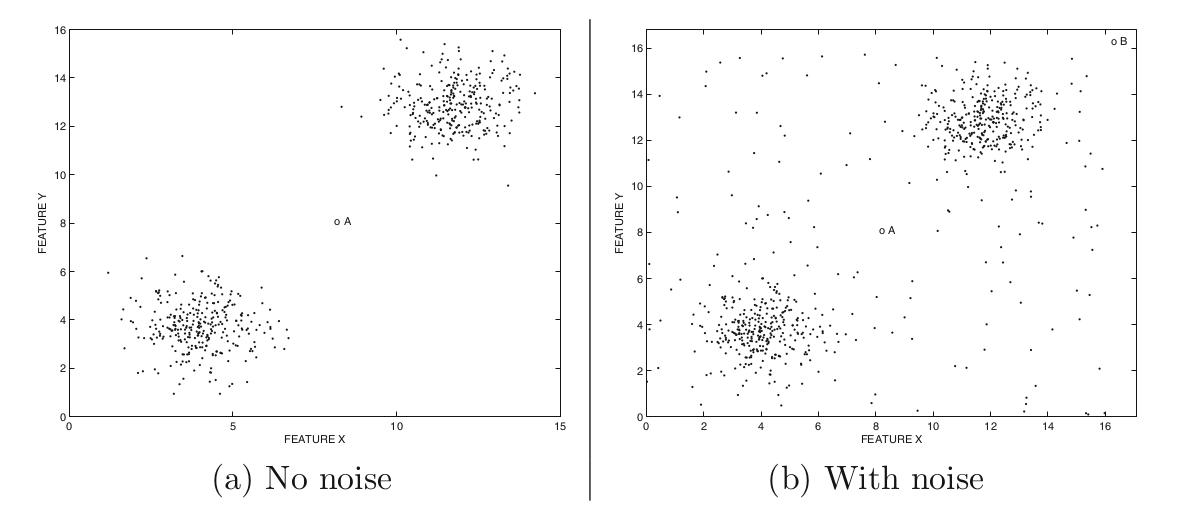
\includegraphics[width=\textwidth]
    {imagenes/ejemplo_basico.jpeg}}
    \caption{\label{fig:my-label} Ejemplo de datos con ruido}
\end{figure}

Como podemos ver en el caso a), la respuesta a si el punto A es una anomalía o no es más fácil. Pero en el caso b) la respuesta
deja de ser tan obvia y empezamos a plantearnos hasta qué punto podemos determinar si un punto es anomalía o no. En datos reales
el problema aumenta, ya que tendremos más dimensiones, cada una con su ruido y una medición podrá desviarse en unas dimensiones y 
en otras seguir el modelo actual. La respuesta ha si hay solución al problema ya no es tan clara. Por tanto, vamos a ver que dos
respuestas se han ofrecido como respuesta a nuestro problema:

\begin{itemize}
    \item \textbf{\textit{Score} de anomalía.} La mayoría de los algoritmos de detección de anomalías responden con una puntuación que cuantifica
    el nivel de ``anomalía" de cada punto de datos. Esta puntuación también se puede utilizar para ordenar los puntos de datos en
    orden para conocer cuáles pueden ser considerados "más" extraños. Esta es una forma muy general cuantificar y resolver el problema,
    que mantiene la información proporcionada por un algoritmo, pero no ofrece una respuesta clara o concisa sobre qué puntos son
    anomalías y cuáles no.
    \item \textbf{Etiqueta binaria.} En este tipo de salida obtenemos una etiqueta binaria por cada punto, indicándonos si se trata de una
    anomalía o no. Existen algunos algoritmos capaces de dar esta respuesta tan precisa, lo normal es usar la puntuación de anomalía. Como
    el resultado que finalmente queremos es una respuesta binaria, lo típico es trasformar las puntuaciones en etiquetas binarias. Para ello,
    normalmente se establecen umbrales en las puntuaciones y este determina puntos que son anomalías. Cuando marcamos un punto como anomalía,
    también estamos perdiendo información del grado de anomalía.
\end{itemize}

En definitiva, podemos decir que estamos enfrentando un problema complicado, cuya decisión de cuando constituye una desviación importante 
para que se considere anomalía no es trivial. A pesar de ello, existen multitud de perspectivas y distintos enfoques para la solución.
En nuestro caso vamos a usar tecnicas basadas en proximidad las cuales explicaremos más adelante.


\section{Motivación}

Este proyecto surge debido a la necesidad de tener una biblioteca de software con algoritmos capaces de afrontar diferentes situaciones de
detección de anomalías. Además, se ha realizado en Python, un lenguaje de programación en alza y muy usado para problemas relacionados con
la computación y la inteligencia artificial. Existe una biblioteca  también
enfocada a la resolución del problema de detección de anomalías\cite{zhaoPyODPythonToolbox2019}, pero este implementa
algoritmos más generalistas y de todos los tipos de enfoque, mientras que en 
nuestro caso queremos enfocarnos y profundizar en el estudio de los algoritmos 
basados en proximidad y aquellos que no son tan conocidos, pero pueden ofrecer un nuevo enfoque y buenos resultados.

La biblioteca se llama \textbf{PyDBOD Python Distances Based Outlier Detector}. Podemos encontrar los repositorios para 
instalar la biblioteca en los repositorios de GitHub \cite{Miki97TFGOutlierDetectionHttps} y en el repositorio de 
PyPI \cite{PyDBODDistancesBased}.